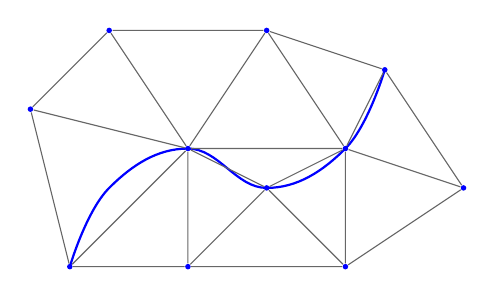
\begin{tikzpicture}
\tikzstyle{mynodestyle} = [
  shape=circle, 
  minimum size=2pt,
  inner sep=0pt,
  fill = blue
]
\tikzstyle{tedge} = [
  draw = black!60
]

\draw [thick, blue]  plot[smooth, tension=.7] coordinates {
  (-1,-1.5) (-0.5,-0.5) (0.5,0) (1.5,-0.5) (2.5,0) (3,1)
};

\node [mynodestyle] (v1) at (0.5,-1.5) {};
\node [mynodestyle] (v2) at (-1,-1.5) {};
\node [mynodestyle] (v3) at (-1.5,0.5) {};
\node [mynodestyle] (v4) at (0.5,0) {};
\node [mynodestyle] (v5) at (-0.5,1.5) {};
\node [mynodestyle] (v6) at (1.5,1.5) {};
\node [mynodestyle] (v7) at (2.5,0) {};
\node [mynodestyle] (v8) at (3,1) {};
\node [mynodestyle] (v9) at (4,-0.5) {};
\node [mynodestyle] (v10) at (2.5,-1.5) {};
\node [mynodestyle] (v11) at (1.5,-0.5) {};

\draw[tedge] (v1) -- (v2) -- (v3) -- (v4) -- (v3) -- (v5) -- (v4) -- (v6) -- (v5);
\draw[tedge] (v6) -- (v7) -- (v8) -- (v6);
\draw[tedge] (v8) -- (v9) -- (v7) -- (v10) -- (v11) -- (v4) -- (v7) -- (v11);
\draw[tedge] (v1) -- (v4) -- (v2);
\draw[tedge] (v9) -- (v10) -- (v1) -- (v11);

\end{tikzpicture}